
\documentclass[a4paper,UKenglish,cleveref, autoref]{oasics-v2019}

\bibliographystyle{plainurl}
\usepackage{booktabs}
\usepackage{fancyvrb}
\fvset{fontsize=\small,commandchars=\\\{\}}


\def\ourtitle{Musikla: Language for Generating Musical Events}
\title{\ourtitle}
\titlerunning{\ourtitle}

\author{Pedro M. Silva}{Dummy University Computing Laboratory, Portugal \and My second affiliation, Country \and \url{http://www.myhomepage.edu} }{johnqpublic@dummyuni.org}{https://orcid.org/0000-0002-1825-0097}{(Optional) author-specific funding acknowledgements}

\author{José João Almeida}%
       {Algoritmi, Departamento de Informática, Universidade do Minho, Braga, Portugal}%
       {jj@di.uminho.pt}%
       {https://orcid.org/0000-0002-0722-2031}
       {}

\authorrunning{Pedro M. Silva and J.\,J. Almeida}
\Copyright{Pedro Miguel Silva, José João Almeida}

\begin{CCSXML}
<ccs2012>
<concept>
<concept_id>10010147.10010178.10010179.10010186</concept_id>
<concept_desc>Computing methodologies~Language resources</concept_desc>
<concept_significance>500</concept_significance>
</concept>
</ccs2012>
\end{CCSXML}

\ccsdesc[500]{Computing methodologies~Language resources}

\keywords{Umbundu, Angola Languages, Morphological Analysis, Spell Checking}

%\funding{This research was partially funded by Portuguese National funds
%(PIDDAC), through the FCT – Fundação para a Ciência e Tecnologia and
%FCT/MCTES under the scope of the projects UIDB/05549/2020 and
%UIDB/00319/2020.  Bernardo Sacanene acknowledges from the Angolan
%govenment his PhD grant, through INAGBE (Instituto Nacional de Gestão
%de Bolsas de Estudos).}

%\nolinenumbers %uncomment to disable line numbering

%Editor-only macros:: begin (do not touch as author)%%%%%%%%%%%%%%%%%%%%%%%%%%%%%%%%%%
\EventEditors{John Q. Open and Joan R. Access}
\EventNoEds{2}
\EventLongTitle{42nd Conference on Very Important Topics (SLATE 2020)}
\EventShortTitle{SLATE 2020}
\EventAcronym{SLATE}
\EventYear{2020}
\EventDate{December 24--27, 2020}
\EventLocation{Little Whinging, United Kingdom}
\EventLogo{}
\SeriesVolume{42}
\ArticleNo{23}
%%%%%%%%%%%%%%%%%%%%%%%%%%%%%%%%%%%%%%%%%%%%%%%%%%%%%%

\begin{document}

\maketitle

\begin{abstract}
  In this paper, we'll discuss a simple approach to integrating musical events, such as notes or chords, into a programming language. First we'll analyze the problem and its particular requirements. Then we will discuss the solution we developed to meet those requirements. Finally we'll analyze the result and discuss possible alternative routes we could've taken.
\end{abstract}

\section{Introduction}
Musikla stands for Music and Keyboard Language. Our goal is to develop a DSL (\textit{Domain Specific Language}) that allows treating musical events as regular data in a programming language. More than generating these musical events offline, we want to be able to easily declare keyboards that map keys to expressions that either mutate the state or play musical events (or even both).

The project can be partitioned in three different, modular layers: inputs, the language, and outputs. While music events can be described as code literals inside our language, they can also originate from many other sources (such as files or physical devices such as pianos). After being processed by our language, they are then emitted as a stream of musical events to the \textbf{Player} component, which then multiplexes those events into however many outputs the user defined.

% TODO Translate diagram to english

\begin{figure}[ht]
  \centering
  {%
  \setlength{\fboxsep}{0pt}%
  \setlength{\fboxrule}{0pt}%
  \fbox{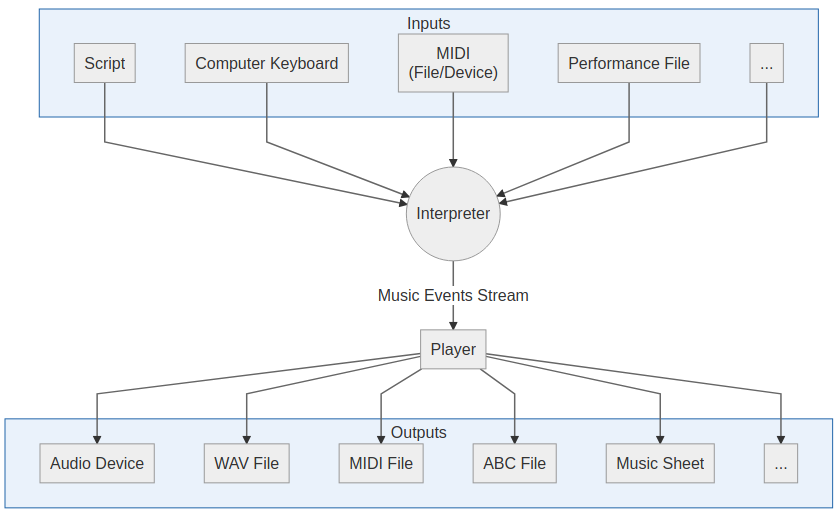
\includegraphics[width=.65\linewidth]{../dissertation/rpd/img/diagram_architecture_en_vertical.png}}%
  }%
  \caption{The three main layers of the project.}
  \label{fig:architecture}
\end{figure}

While the development of both the input and output layers, as well as their many respective components, presents by itself many interesting challenges that could be discussed, we will instead focus this paper on the aspects of the middle layer: the \textit{interpreter}, while ackowledging the existence (and their effects) of the layers that wrap around it.

As such, the problem of developing the interpreter can be divided into two parts: the syntax used for describing the notes and the operators that compose them inside the language; and the semantics of the generated events, how they are stored in memory, and how their temporal properties (start time and duration) are handled without forcing the programmer/user to always manually type them. 

Designing the syntax for describing those musical expressions, especially given our strong desire to make those musical expressions first class citizens like other primitive data types in most programming languages (such as numbers, strings or arrays are), did unearth some challenges. To minimize the learning curve for new users, and avoid reinventing the wheel, we decided to adopt a subset of the very popular note declaration syntax from the ABC Notation project\cite{AbcNotation} and integrate it with our language.

As for the execution model, we decided to go with a tree-walker interpreter\cite{CraftingInterpreters}. Altough computationally slower than other alternatives (such as a bytecode virtual machine), the ease of implementation allowed us to prototype and develop features extremely fast. And with a more mature and stable language in the future, there is always the potential to rewrite the interpreter if performance or latency ever reveal themselves as potential problems.


The simplest way of generating such musical events in a programming language is to use already common, \textit{low-level}, programming mechanisms, such as using a procedural approach where the user creates each event manually by calling a function and providing as parameters all the events' information, such as it's timestamp and duration. This is the approach used by some of the existing languages in this space, such as \textit{SonicPi}\cite{Aaron2014TemporalSF}.

\begin{lstlisting}[caption={Example of a hypothetical imperative API for creating events},label=list:1,captionpos=t,abovecaptionskip=-\medskipamount]
play_note( 0, 100, 'A' );
play_note( 100, 50, 'B' );
play_note( 150, 200, 'C' );
\end{lstlisting}

Instead we decided to follow a more \textit{functional} approach, with custom syntax and operators, as well as the hability to describe those events in a single expression. Musical events are treated as sequences, and as such can be stored in variables, passed around inside functions and trasformed. So, for musical events, we will be exploring a way to define them in code, as \textit{musical literals}.

\begin{lstlisting}[caption={Our proposed declarative syntax that calculates timings implicitly},label=list:2,captionpos=t,abovecaptionskip=-\medskipamount]
play( A B/2 C2 );
\end{lstlisting}

\section{The Problem and its Requirements}
There are two important requirements we need to consider when evaluating possible solutions to this problem: the ability to produce music interactively, and to produce music lazily.

The first requirement, \textbf{Interactivity}, relates to our goal of not only being able to generate music offline, but also in a live environment: give the user the ability to program several snippets of musical events, and then control them through a virtual keyboard or through other interactive means.

The second requirement, \textbf{Laziness}, refers to a concept that is familiar in functional programming languages: values are generated when we need them, not earlier. In our case, this implies that a musical sequence could be potentially infinite (like an infinite repetition of some arrangement). If playing this music live, the musician could determine to stop this arrangement sooner or later.

Given these two requirements, we can conclude we \textbf{cannot} generate all music events at the start and then sort them to play them in order. Because of that, the events must always be sorted already.

\begin{lemma}[Total Order]
\label{lemma:total-order} All operators must return a sequence of events that respects our time unit's total order.
\end{lemma}

\paragraph*{Data Model}
The basic premise is that expressions can generate a special data type: \textbf{Music}. Music is simply a sequence (or stream) of ordered musical events.

A musical \textbf{Event} can be one of many things, such as a \textit{note}, a \textit{chord}, or even more implementation-specific events like MIDI messages\cite{Loy1985MusiciansMA}. While all events must have a start time, some events can be instantaneous (events with a duration of zero time units).

The time unit used does not need to be a common time measure, like seconds or milliseconds, and can be really anything so long as it has a \textbf{total order}.

\paragraph*{Operators}
Operators are special operations defined at the syntactic level that allow \textit{music} to be composed in different ways, such as concatenated, parallelized or repeated. Many of these operators can have equivalent functions available through the language that provide more costumization (such as a parallel function that stops when the smaallest operand stops, instead of the longest).

\begin{description}
    \item[Concatenation] \verb|Music1 Music2 ... MusicN|
    
        \textbf{type} \verb|List[Music] -> Music|
    \item[Parallel] \verb'Music1 | Music2 | ... | MusicN'
        
        \textbf{type} \verb|List[Music] -> Music|
    \item[Repetition] \verb'Music * Integer'
    
        \textbf{type} \verb|Music, Integer -> Music|
    \item[Arpegio] \verb'Chord * Music'
        
        \textbf{type} \verb|Chord, Music -> Music|
    \item[Transpose] \verb'Music + Integer' \textit{and} \verb'Music - Integer'
    
        \textbf{type} \verb|Music, Integer -> Music|
\end{description}


It is also useful to estabilish that while most operators work on sequences of musical events, they can also accept a singular event as their argument: one event can be trivially converted into a sequence of one element. Such ocorrence is so common and trivial that the conversion should therefore be implicit whenever necessary.

\paragraph*{Grids}
Another type available in our language are grids. Also known in most music applications as the process of quantization \cite{Quantization}. The reason it is so useful in our language is that when receiving input as musical events from a live keyboard, their timings are naturally more prone to having small discrepancies that can become more apparent when we then mix them with generated musical events (which have precise timings).


Having events always aligned with such a grid can also make computations and transformations of such events easier and simpler, which is always a plus for our language.


\begin{description}
    \item[Create a grid] \verb|Grid(size)|
    
        \textbf{type} \verb|Fraction -> Grid|
    \item[Aligning] \verb'grid::align(music)'
        
        \textbf{type} \verb|Grid, Music -> Music|
    \item[Compose Grids] \verb'Grid::compose(grid1, grid2, ..., gridN)'
        
        \textbf{type} \verb|List[Grid] -> Grid|
\end{description}

We can see that apart from the basic operations of creating a grid and aligning events to said grid, we also want the ability to compose multiple grids (of different precisions). We will approach this matter in more detail later.

\paragraph*{Keyboards}
A core part of the language is our hability to declare keyboards, which we can describe as mappings between \texttt{Keys} and \textit{Musical Expressions}.

Each expression can mutate the state (changing variables or calling functions), return some music (sequence of musical events) to be played, or both.

Some of the operations we want to be able to perform with keyboards are as follows:

\begin{description}
    \item[Create a keyboard] \verb|keyboards\create()|
    
        \textbf{type} \verb|() -> Keyboard|
    \item[Binding a Key] \verb'keyboard::register(key, expression)'
        
        \textbf{type} \verb|Keyboard, Key, Expression -> Keyboard|
    \item[Mapping a keyboard] \verb'keyboard::map(transformer)'
        
        \textbf{type} \verb|Keyboard, ( Music -> Music ) -> Keyboard|
    \item[Aligning with a Grid] \verb'keyboard::with_grid(grid)'
        
        \textbf{type} \verb|Keyboard, Grid -> Keyboard|    
\end{description}


\section{Implementation}
The reference implementation for this system is written in Python, although the approach here should be language agnostic.

One of the features that Python boasts (but are certainly not exclusive to it) that have eased our implementation of the language are generators\cite{PEP255}. They integrate very nicely into both our concept of emitting musical events as sequences (or iterators, as they are called in Python and other languages), as well as into our concept of laziness, where events are generated on demand when needed, and thus infinite musical sequences can be handled easily.

\paragraph*{Context State}
To keep track of the \textit{cursor} (the current timestamp where the next event should start) each operator in our language is implemented as a function call that receives an implicit \texttt{Context} object. While here we'll mostly focus just on the methods related to time management provided by the context, it can be used to store other types of information, like the default length of a musical note, for instance, to avoid forcing the user to type it out all the time, or the tempo at which it is to be played.

It is important to keep in mind that there might be more than one context in execution at the same time. This can be most obvious with the use of the parallel operator, where each operand must run concurrently (and thus could not share the same context).

Let's describe what kinds of functionality our context should provide.

\begin{description}
    \item[cursor(ctx)] Return the current cursor position
    \item[seek(ctx, time)] Advance the cursor to the given position
    \item[fork(ctx)] Clone the parent context and return the new one. Allows multiple concurrent contexts to be used
    \item[join(parent, child)] If the child's cursor is ahead, make the parent context catch up
\end{description}

\subsection{Operators}

\paragraph*{Basic Events}
The basic building block of our system are the \textbf{Note}, \textbf{Chord} and \textbf{Rest} events. We can use the current \textit{context} to determine the event's timestamp, as well as it's default duration (in case the user does not explicitly state one). Any event(s) that is/are not captured in a variable or passed to a function are implicitly played.

\begin{lstlisting}[caption={Creating a Note Event},label=list:3,captionpos=t,abovecaptionskip=-\medskipamount]
c'1/4
\end{lstlisting}

\paragraph*{Concatenation}
We've seen how single events' creation is handled. Now it is important for us to see how we can combine those events together. And probably the most straightforward operator of all, concatenation, it simply consumes each event. Each event, as we've seen before, is responsible for seeking the context depending on the event's duration.
\begin{lstlisting}[caption={Snippet of the song \textit{Wet Hands} by C418},label=list:4,captionpos=t,abovecaptionskip=-\medskipamount]
S4/4 T74 L/8 V90;
A, E A B ^c B A E D ^F ^c e ^c A3;
\end{lstlisting}

\begin{figure}[ht]
  \centering
  {%
  \setlength{\fboxsep}{0pt}%
  \setlength{\fboxrule}{0pt}%
  \fbox{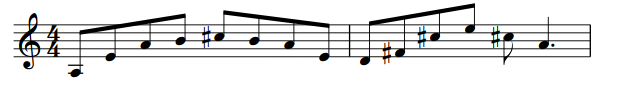
\includegraphics[width=.85\linewidth]{../code/musikla/musikla/examples/paper/concatenation2.png}}%
  }%
  \caption{Generated music sheet for concatenation\protect\footnotemark, audio version available \href{https://drive.google.com/open?id=1TP4lcul81s8iMCUFmD3HKnSpeftCzKT0}{\underline{here}}.}
  \label{fig:concatenation}
\end{figure}

\footnotetext{Rendered with \$ABC\_UI. Some hand made changes made for clarity.}


\paragraph*{Repetition}
The repetition operand is in a way very similar to the concatenation operator. It makes sense, since repeating any kind of music pattern $N$ times could be thought as a particular case of as concatenation where there are $N$ operands, all representing the same musical pattern.

\begin{lstlisting}[caption={Intro to Westworld's Theme by Ramin Djawadi},label=list:5,captionpos=t,abovecaptionskip=-\medskipamount]
I1 S6/8 T140 L/8 V90;
A*11 G F*12
\end{lstlisting}

\begin{figure}[ht]
  \centering
  {%
  \setlength{\fboxsep}{0pt}%
  \setlength{\fboxrule}{0pt}%
  \fbox{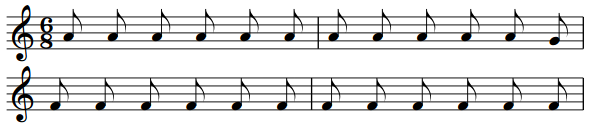
\includegraphics[width=.85\linewidth]{../code/musikla/musikla/examples/paper/repetition2.png}}%
  }%
  \caption{Generated music sheet for repetition, audio version available \href{https://drive.google.com/open?id=1IIm8PQkLsNFMK9MNSVubJSG6SP6KwhPL}{\underline{here}}.}
  \label{fig:repetition}
\end{figure}

\paragraph*{Parallel}
The parallel operator enables playing multiple sequences of musical events simultaneously. However our events are emitted as a single sequence of ordered events, thus requiring merging the multiple sequences into a single one, while maintaining the properties of laziness and order. The operator assumes that each of its operands already maintains those properties on their own, and so is only in charge of making sure the merged sequence does so as well. With this in mind, it relies on a custom \textit{merge sorted} algorithm for iterables (not related to the most common merge sort algorithm by John von Neumann).

\begin{lstlisting}[caption={Snippet of the song \textit{Soft to Be Strong} by Marina},label=list:6,captionpos=t,abovecaptionskip=-\medskipamount]
T120 V70 L1;
r/4 ^g/4 ^g/4 ^g/4   ^f/2 e/8 ^d3/8   ^c2 | [^Cm] [BM]  [AM] [BM] 
\end{lstlisting}

\begin{figure}[ht]
  \centering
  {%
  \setlength{\fboxsep}{0pt}%
  \setlength{\fboxrule}{0pt}%
  \fbox{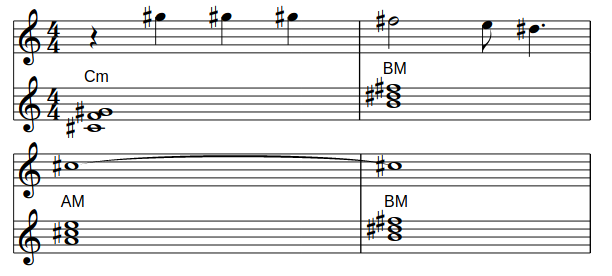
\includegraphics[width=.85\linewidth]{../code/musikla/musikla/examples/paper/parallel2.png}}%
  }%
  \caption{Generated music sheet for parallel, audio version available \href{https://drive.google.com/open?id=1ENTm3hZonYHyQIOgRZ8TQ1Qz-AfRLt2I}{\underline{here}}.}
  \label{fig:parallel}
\end{figure}


The merge sorted function receives $N$ operands and creates a buffer with the size $N$. For each operand it \textit{forks} the context, so that they can execute concurrently and each will mutate their own context only. It then requests one single event for each operand.

After the buffer is prefilled (meaning it has at least one event for all non-empty operands), the algorithm finds the earliest event stored in the it. Let's assume it is stored in the $K$ index of the buffer, with $K < N$. The method emits the value stored in \texttt{buffer[K]} and then fills requests the next event from the $K$ operand (storing \texttt{null} if the operand has no more events to emit). It then repeats this step until all operands have been drained.

\subsection{Integration in a Programming Environment}
Apart from generating musical events from somewhat static instructions, our goal is to have those events integrate into a programming language in the same way integers, floats, strings and booleans do: as data that can be stored, passed around and manipulated. This, of course, must still retain all the properties we've laid out for our sequences of events: being lazy and always being ordered.

\paragraph*{Variables and Functions}
All expressions that are assigned to a variable run in a forked context, with it's cursor set to zero initially. Musical expressions inside variables are still lazy (meaning they only calculate each musical event when the variable is first used, not declared) but the events are cached to prevent the calculations from being performed every time. This cache is then garbage collected when the variable is no longer in use.

Since events declared inside variables have their start time set relative to zero, it needs to be calculated each time the variable is used to replace it with the correct value. This highlights an important aspect of our language: the need for each musical event to be immutable, and any changes made to them to actually be implemented as new instances of the event.

This works well enough because those events are very lightweight objects, and the benefits of not having their values mysteriously changed midway during execution outweight the small cost of a possible unnecessary allocation of an event that would only be used in one place instead of many.

Function calls, on the other hand, pass the current context to the inside of the function, so  that any events played there now their correct times.

When integrating functions into our language, we decided to keep the semantics simple. Emitting musical events inside a function is similar to its return value being an iterator that gives out the emitted events on demand. This means that a value cannot both emit musical events, while also returning other values manually through a return statement.

There is no syntactic marker to distinguish regular functions from musical-emitting ones. Instead, the language runtime starts executing each function as a regular one, and automatically switches its execution mode into a generator-like implementation once the first event is emitted. Any return statements that are evaluated after this point must have no value (thus preserving the feature to early-stop a function). If they do try to return a custom value, a runtime exception is triggered.

Here we can see a small snippet of the beginning of \textit{Fugue 2 in C minor in Book I of the J.S. Bach’s Well-Tempered Clavier}, and how using functions and variables can help us visualize the structure behind music.

\begin{lstlisting}[caption={Example of repeating the same note},label=list:7,captionpos=t,abovecaptionskip=-\medskipamount]
fun fugue ( $subj, $resp ) => 
    ( $subj $resp | stretch( r, $subj ) ( $subj + 7 ) );

S8/4 T140 L/4 V120;

$subj = r c/2 B/2 c G _A c/2 B/2 c d
        G c/2 B/2 c d F/2 G/2 _A2 G/2 F/2;

$resp = E/2 c/2 B/2 A/2   G/2 F/2 _E/2 D/2   C _e d c
        _B A _B c   ^F G _A F;

play( fugue( $subj, $resp ) );
\end{lstlisting}


\begin{figure}[ht]
  \centering
  {%
  \setlength{\fboxsep}{0pt}%
  \setlength{\fboxrule}{0pt}%
  \fbox{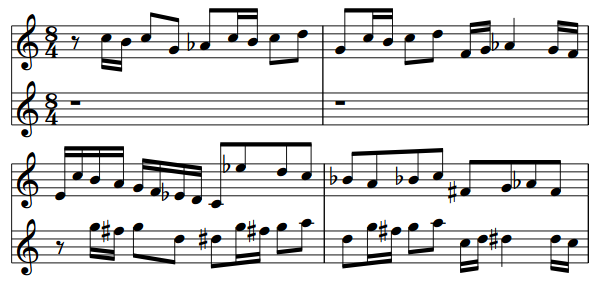
\includegraphics[width=.85\linewidth]{../code/musikla/musikla/examples/paper/fugue.png}}%
  }%
  \caption{Generated music sheet for fugue example, audio version available \href{https://drive.google.com/open?id=1dIfvnhhKn73Vpp0W6ss6RLsv6PQ_HFTF}{\underline{here}}.}
  \label{fig:fugue}
\end{figure}
% https://drive.google.com/open?id=1-igVwdhXMxOSE1cMg_8HimDOXMhsY9US

\paragraph*{Grids}
To define a grid there is only one parameter required: the length of it's cells. When aligning musical events, anything that falls inside each cell will be pushed to the closest edge of the cell.

Grids are highly customizable too, however. They have multiple parameters, such as \texttt{forgiveness} and \texttt{range}, that determine when an event is affected by the grid (depending on how close it's start time is to the edge of the cell). Each parameter can even be customized separately for the left and right sides of the cell's edge.

Let's take a look at an example of a grid. In this example the grid has a cell size of \textbf{1}. We define the same values for both left and right sides just for the sake of this demonstration, but each side could have different values.

\begin{lstlisting}[caption={Declaring a grid},label=list:8,captionpos=t,abovecaptionskip=-\medskipamount]
$grid = Grid( 1,
    forgiveness_left = 125, # 1/8
    range_left = 375, # 3/8
    forgiveness_right = 125, #1/8
    range_right = 375 # 3/8
);
\end{lstlisting}

\begin{figure}[ht]
  \centering
  {%
  \setlength{\fboxsep}{0pt}%
  \setlength{\fboxrule}{0pt}%
  \fbox{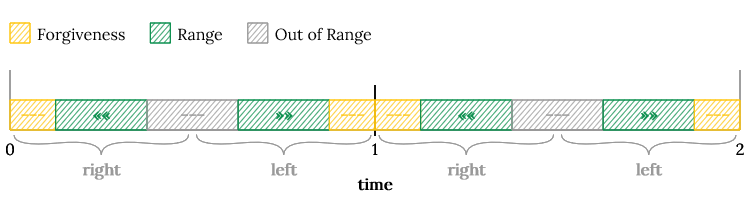
\includegraphics[width=.95\linewidth]{./img/grids.png}}%
  }%
  \caption{Representation of two cells from this grid.}
  \label{fig:grid}
\end{figure}

We can see in this timeline two cells (each with a size of 1). Any events that fall in the yellow and grey areas are ignored (meaning their timestamps are not changed) while events in the green areas are pushed to whatever edge is closest. But even this behavior can be customized, forcing events to always go to the previous edge cell, or always to the next.

It is then trivial to see how we could compose multiple grids in sequence, each with different ranges (green areas) that capture different events and align them accordingly.

\paragraph*{Keyboards}
Finally we can combine all the systems we've described above, from musical expressions, grids, variables and functions, and devise a compact way of describing virtual keyboards.

To make the process of designing keyboards less verbose, we've added syntactic sugar to this process, that is translated in the background to regular function calls registering each key binding.

While a picture maybe worth a thousand words, a good example is worth maybe even more. So here we can take a brief look at the workflow for defining two keyboards (that are active at the same time). The first keyboard has all the musical keys (the chords and single notes we want), all aligned by a custom grid.

The second keyboard binds to the up and down arrow keys and allow us to change the virtual instrument through which we play the sounds of the notes in the keyboard (those instruments can be identified by an integer and usually follow the General MIDI standard\cite{GeneralMIDI}).

\begin{lstlisting}[caption={Creating a keyboard that can play multiple instruments},label=list:9,captionpos=t,abovecaptionskip=-\medskipamount]
$inst = 0;

fun spin_instrument ( ref $instrument, $change ) {
    $instrument = $instrument + $change;
    
    setinstrument( $instrument );
};

@keyboard {
    a: [^Cm];   s: [BM];    d: [AM];    f: [EM];    g: [^Fm];
    1: ^c;      2: ^d;      3: e;       4: ^f;      5: ^g;
    6: b;       7: ^c';     8: ^d';     9: e';
}::with_grid( Grid( 1 / 16 ) );

@keyboard {
    up: spin_instrument( $inst, 1 );
    down: spin_instrument( $inst, -1 );
};
\end{lstlisting}

Keyboards are objects (that we could save in a variable for example) and that can perform many operations, like unions and intersections, or maps and filters. They can be enabled and disabled at runtime, and their keys can be simulated to be pressed and released.

More than that, we don't need to restrict ourselves to computer keyboards. We can for instance, define bindings between MIDI events and musical expressions, so that when we connect a piano keyboard to our computer, we can use each piano key to play more than a single note.

Since like we've seen keyboard keys are not limited to computer keyboards, we can imagine the possibilities of events we could listen to: knobs, mouse buttons, the mouse scroll wheel. We could even create an event that could, for example, listen on a socket and trigger when a message is received, allowing in that way our musical applications to be controlled remotely.

The result is that our keyboards are extremely extensible and allow for a great deal of creativity. And thanks to our tight integration with the Python language, those extensions can be easily integrated and don't require hacking the source code or recompiling the application.

\section{Results Discussion}
\label{sec:conclusions}

To solve our problem of keeping track of the timing implicitly for each event created, we decided to pass around a context variable. There were other possible solutions, like keeping this data in some sort of global variable. Our approach does give us some advantages, such as beeing able to have multiple contexts in play at the same time. It does have drawbacks, too. Every function defined in our language must receive this context to be able to create events at the appropriate time. However, functions defined in Python do not expect this parameter. Therefore, special conversions must be made when exchanging values between both languages.

Also, our solution to have variables just offset the timings of each event they contain every time those variables are used simplifies the process of integrating variables into our existing semantics of music generation. This solution, however, does not answer other questions unrelated to the timing, such as: should events stored in variables use the musical instrument set when they were declared, or when the variable was used?

However, this early work already provides a solid foundation for a musical \textit{DSL} that while dynamic (with variables, functions and control structures) integrates very well with established musical standards such as the MIDI protocol and others.


\bibliography{references}

\end{document}
